

\documentclass[
    % -- opções da classe memoir --
    openany,
    12pt,               % tamanho da fonte
    twoside,            % para impressão em verso e anverso. Oposto a oneside
    a4paper,            % tamanho do papel. 
    english,            % idioma adicional para hifenização
    brazil,             % o último idioma é o principal do documento
    ]{abntex2}


% ---
% Pacotes fundamentais 
% ---
\usepackage{cmap}               % Mapear caracteres especiais no PDF
\usepackage{lmodern}            % Usa a fonte Latin Modern
\usepackage[T1]{fontenc}        % Selecao de codigos de fonte.
\usepackage[utf8]{inputenc}     % Codificacao do documento (conversão automática dos acentos)
\usepackage{lastpage}           % Usado pela Ficha catalográfica
\usepackage{indentfirst}        % Indenta o primeiro parágrafo de cada seção.
\usepackage{color}              % Controle das cores
\usepackage{graphicx}           % Inclusão de gráficos
\usepackage{xspace}
\usepackage{fourier} 
\usepackage{array}
\usepackage{makecell}
\usepackage{graphics}
\usepackage{float}

% ---

% Pacotes extras
\usepackage[table,xcdraw]{xcolor}   % Inclusão de cores em tabelas
\usepackage{todonotes}
\usepackage{multirow}
\usepackage{pdfpages}
\usepackage{pgfgantt}
\usepackage{changepage}
\usepackage{hyperref}
\usepackage{seqsplit}
\usepackage{caption}

% Acronyms
\usepackage[acronym,nowarn]{glossaries}

\glsdisablehyper
%==============================================================================
% Computer Architecture
%=============================================================================

\newcommand{\manycore}{\textit{manycore}\xspace}
\newcommand{\manycores}{\textit{manycores}\xspace}

% Manycores
\newcommand{\scc}{\textit{Intel Single-Cloud Computer}\xspace}
\newcommand{\xeonphi}{\textit{Intel Xeon Phi}\xspace}
\newcommand{\tilegx}{\textit{Tilera TILE-Gx100}\xspace}
\newcommand{\tilepro}{\textit{Tilera TILE64}\xspace}
%\newcommand{\mppa}{\textit{Kalray MPPA-256}\xspace}
\newcommand{\taihulight}{\textit{Sunway SW26010}\xspace}
\newcommand{\epiphany}{\textit{Adapteva Epiphany}\xspace}
\newcommand{\optimsoc}{\textit{OpTiMSoC}\xspace}

\newacronym{mppa-256}{MPPA-256}{\textit{Kalray MPPA-256}}
	\newcommand{\mppa}{\gls{mppa-256}\xspace}

% Taxonomy
\newacronym{mimd}{MIMD}{\textit{Multiple Instruction Multiple Data}}
	\newcommand{\mimd}{\gls{mimd}\xspace}
\newacronym{simd}{SIMD}{\textit{Single Instruction Multiple Data}}
	\newcommand{\simd}{\gls{simd}\xspace}
\newacronym{numa}{NUMA}{\textit{Non-Uniform Memory Access}}
	\newcommand{\numa}{\gls{numa}\xspace}
\newacronym{norma}{NoRMA}{\textit{No Remote Memory Access}}
	\newcommand{\norma}{\gls{norma}\xspace}
\newacronym{amp}{AMP}{\textit{Asymmetric Multi-Processing}}
	\newcommand{\amp}{\gls{amp}\xspace}
\newacronym{gpu}{GPU}{\textit{Graphics Processing Unit}}
	\newcommand{\gpu}{\gls{gpu}\xspace}
	\newcommand{\gpus}{\glspl{gpu}\xspace}
\newacronym{fpga}{FPGA}{\textit{Field Programmable Gate Array}}
	\newcommand{\fpga}{\gls{fpga}\xspace}
	\newcommand{\fpgas}{\glspl{fpga}\xspace}
\newacronym{mpsoc}{MPSoC}{\textit{Multiprocessors System-on-Chip}}
	\newcommand{\mpsoc}{\gls{mpsoc}\xspace}
	\newcommand{\mpsocs}{\glspl{mpsoc}\xspace}

% Core
\newacronym{pe}{PE}{\textit{Processing Element}}
	\newcommand{\pe}{\gls{pe}\xspace}
	\newcommand{\pes}{\glspl{pe}\xspace}
\newacronym{rm}{RM}{\textit{Resource Manager}}
	\newcommand{\rman}{\gls{rm}\xspace}
	\newcommand{\rmans}{\glspl{rm}\xspace}

% Memory
\newacronym{mmu}{MMU}{\textit{Memory Management Unit}}
	\newcommand{\mmu}{\gls{mmu}\xspace}
	\newcommand{\mmus}{\glspl{mmu}\xspace}

\newacronym{spd}{SPM}{\textit{Scratchpad Memory}}
	\newcommand{\spd}{\gls{spd}\xspace}
\newacronym{dma}{DMA}{\textit{Direct Memory Access}}
	\newcommand{\dma}{\gls{dma}\xspace}

\newacronym{rma}{RMA}{\textit{Remote Memory Access}}
	\newcommand{\rma}{\gls{rma}\xspace}

% Interconnects
\newacronym{noc}{NoC}{\textit{Network on Chip}}
	\newcommand{\noc}{\gls{noc}\xspace}
	\newcommand{\nocs}{\glspl{noc}\xspace}
\newacronym{cnoc}{C-NoC}{\textit{Control NoC}}
    \newcommand{\cnoc}{\gls{cnoc}\xspace} 
\newacronym{dnoc}{D-NoC}{\textit{Data NoC}}
	\newcommand{\dnoc}{\gls{dnoc}\xspace}     

%==============================================================================
% Operating Systems
%=============================================================================

\newacronym{posix}{POSIX}{\textit{Portable Operating System Interface}}
	\newcommand{\posix}{\gls{posix}\xspace}

\newacronym{api}{API}{\textit{Application Programming Interface}}
	\newcommand{\api}{\gls{api}\xspace}
	\newcommand{\apis}{\glspl{api}\xspace}

% Kernels
\newcommand{\linux}{\textit{GNU/Linux}\xspace}
\newcommand{\unix}{\textit{Unix}\xspace}
\newcommand{\rtems}{\textit{RTEMS}\xspace}
\newcommand{\bsd}{\textit{BSD}\xspace}
\newcommand{\nodeos}{\textit{NodeOS}\xspace}
\newacronym{fos}{FOS}{\textit{Factored Operating System}}
	\newcommand{\fos}{\gls{fos}\xspace}
\newacronym{lfour}{L4}{\textit{L4 Microkernel}}
	\newcommand{\lfour}{\gls{lfour}\xspace}
\newacronym{nos}{nOS}{\textit{Nano-Sized Operating System}}
	\newcommand{\nos}{\gls{nos}\xspace}

\newacronym{ipc}{IPC}{\textit{Inter-Process Communication}}
	\newcommand{\ipc}{\gls{ipc}\xspace}

\newacronym{qos}{QoS}{\textit{Quality of Service}}
	\newcommand{\qos}{\gls{qos}\xspace}

\newacronym{hal}{HAL}{\textit{Hardware Abstraction Layer}}
	\newcommand{\hal}{\gls{hal}\xspace}

%==============================================================================
% High Performance Computing
%=============================================================================

\newacronym{hpc}{HPC}{\textit{High-Performance Computing}}
	\newcommand{\hpc}{\gls{hpc}\xspace}

% Runtimes
\newcommand{\openmp}{OpenMP}
\newcommand{\openmpi}{OpenMPI\xspace}

\newacronym{pgas}{PGAS}{\textit{Partitioned Global Address Space}}
	\newcommand{\pgas}{\gls{pgas}\xspace}

\newacronym{mpi}{MPI}{\textit{Message Passing Interface}}
	\newcommand{\mpi}{\gls{mpi}\xspace}

%==============================================================================
% Other
%=============================================================================

\newacronym{rmem}{RMem}{\textit{Remote Memory}}
	\newcommand{\rmem}{\gls{rmem}\xspace}

\newcommand{\ie}{i.e.,\xspace}
\newcommand{\etal}{\textit{et al.}\xspace}

\newacronym{iid}{i.i.d}{\textit{Independent and Identically Distributed}}
	\newcommand{\iid}{\gls{iid}\xspace}

\newacronym{anova}{ANOVA}{\textit{Analysis of Variance}}
	\newcommand{\anova}{\gls{anova}\xspace}

\newacronym{mit}{MIT}{\textit{Massachusetts Institute of Technology}}
	\newcommand{\unimit}{\gls{mit}\xspace}

\newacronym{lig}{LIG}{\textit{Laboratoire d'Informatique de Grenoble}}
    \newcommand{\lig}{\gls{lig}\xspace}

\newacronym{lapesd}{LaPeSD}{\textit{Distributed Systems Research Laboratory}}
    \newcommand{\lapesd}{\gls{lapesd}\xspace}

\newacronym{ufsc}{UFSC}{{Universidade Federal de Santa Catarina}}
    \newcommand{\ufsc}{\gls{ufsc}\xspace}
	
\newcommand{\cpcluster}{\textit{Compute Cluster}\xspace}
\newcommand{\cpclusters}{\textit{Compute Clusters}\xspace}
\newcommand{\iocluster}{\textit{IO Cluster}\xspace}
\newcommand{\ioclusters}{\textit{IO Clusters}\xspace}

\newcommand{\capb}{CAP Bench\xspace}

\newacronym{ASYNC}{ASYNC}{\textit{MPPA Asynchronous Communication}}
\newcommand{\async}{\gls{ASYNC}\xspace}

\newacronym{cc}{CC}{\textit{cluster} de computação}
	\newcommand{\cc}{\gls{cc}\xspace}

\newacronym{ccs}{CCs}{\textit{clusters} de computação}
	\newcommand{\ccs}{\gls{ccs}\xspace}
   
\newacronym{io}{E/S}{Entrada e Saída}
    \newcommand{\io}{\gls{io}\xspace}

% Code Style
\usepackage{xcolor}
\usepackage{listings}

\definecolor{mGreen}{rgb}{0,0.6,0}
\definecolor{mGray}{rgb}{0.5,0.5,0.5}
\definecolor{mPurple}{rgb}{0.58,0,0.82}
\definecolor{backgroundColour}{rgb}{0.95,0.95,0.92}

\lstset{%
  escapeinside={(*}{*)},%
}

\lstdefinestyle{CStyle}{
    backgroundcolor=\color{backgroundColour},   
    commentstyle=\color{mGreen},
    keywordstyle=\color{magenta},
    numberstyle=\tiny\color{mGray},
    stringstyle=\color{mPurple},
    basicstyle=\footnotesize,
    breakatwhitespace=false,         
    breaklines=true,                 
    captionpos=b,                    
    keepspaces=true,                 
    numbers=left,                    
    numbersep=5pt,                  
    showspaces=false,                
    showstringspaces=false,
    showtabs=false,                  
    tabsize=2,
    language=C
}

\lstdefinestyle{BashStyle}{
    breakatwhitespace=false,         
    breaklines=true,                 
    captionpos=b,                    
    keepspaces=true,                 
    numbers=left,                    
    numbersep=5pt,                  
    showspaces=false,                
    showstringspaces=false,
    showtabs=false,                  
    tabsize=2,
    language=bash
}

% ---
% Pacotes de citações
% ---
%\usepackage[brazilian,hyperpageref]{backref}    % Paginas com as citações na bibl
\usepackage[alf]{abntex2cite}                    % Citações padrão ABNT

% ---
% Informações de dados para CAPA e FOLHA DE ROSTO
% ---
\titulo{INE5429 - 2021.2 - Trabalho final em grupo}
\autor{David Grunheidt Vilela Ordine - 16202253}
\local{Florianópolis}
\data{2021}
\instituicao{%
  Universidade Federal de Santa Catarina
  \par
  Departamento de Informática e Estatística
  \par
  Ciência da Computação}

% ---
% Configurações de aparência do PDF final

% alterando o aspecto da cor azul
\definecolor{blue}{RGB}{41,5,195}

% informações do PDF
\makeatletter
\hypersetup{
        %pagebackref=true,
        pdftitle={\@title}, 
        pdfauthor={\@author},
        pdfsubject={\imprimirpreambulo},
        pdfcreator={LaTeX with abnTeX2},
        pdfkeywords={abnt}{latex}{abntex}{abntex2}{trabalho acadêmico}, 
        hidelinks,
        colorlinks=true,           % false: boxed links; true: colored links
        linkcolor=blue,             % color of internal links
        citecolor=blue,             % color of links to bibliography
        filecolor=magenta,          % color of file links
        urlcolor=blue,
        bookmarksdepth=4
}
\makeatother
% --- 

% --- 
% Espaçamentos entre linhas e parágrafos 
% --- 

% O tamanho do parágrafo é dado por:
\setlength{\parindent}{1.3cm}

% Controle do espaçamento entre um parágrafo e outro:
\setlength{\parskip}{0.2cm}  % tente também \onelineskip

% ---
% compila o indice
% ---
\makeindex
% ---

% ----
% Início do documento
% ----
\begin{document}

% Retira espaço extra obsoleto entre as frases.
\frenchspacing 

% ---
% Folha de rosto
% ---
\imprimirfolhaderosto*
% ---

% ---
% inserir o sumario
% ---
\pdfbookmark[0]{\contentsname}{toc}
\tableofcontents
\cleardoublepage
% ---


% ----------------------------------------------------------
% ELEMENTOS TEXTUAIS
% ----------------------------------------------------------
\textual

\chapter{Referencial teórico}
\label{cap:ref-teorico}

\subsection{Certificação digital}
\label{cap:cert-digital}
Certificado digital pode ser considerado como a identidade eletrônica de uma pessoa ou empresa. Basicamente, ele funciona como uma carteira de identificação digital virtual, onde é possível assinar documentos a distancia com o mesmo valor judiciário de uma assinatura física. 

A partir do certificado, é possível fazer uma ligação entre uma certa entidade e uma chave pública. Quando se fala de Infraestrutura de Chaves Públicas (ICP), a Autoridade Certificadora (AC) que o emite certo certificado é também responsável por assinalo. Já no caso de um modelo de Teia de Confiança (Web of trust) como o PGP, a entidade e todos os outros que confiam nela assinam o certificado. As assinaturas de ambos os exemplos são atestamentos feitos por uma entidade que confia nos dados do certificado. 

No certificado é incluso, dentre outros:
\begin{itemize}
\item{Assinatura das entidades ou ACs que validaram que a chave pública do certificado confere com as informações contidas neste.}
\item{O período de validade do certificado.}
\item{A chave pública associada a chave privada, a qual a segunda somente a entidade especificada no certificado possui.}
\item{Url do "centro de revogação" (download da LCR ou para uma consulta OCSP).}
\item{Informações sobre a entidade para o qual o certificado foi emitido (email, CPF/CNPJ, nome, PIS etc.).}
\end{itemize}

\subsection{SSL/TLS}
\label{cap:ssl-tls}

\textbf{SSL} é a abreviação para \textit{Secure Sockets Layer}, onde existe uma segurança digital que permite a comunicação criptografada entre um determinado site e um navegador. Atualmente o SSL se encontra depreciado e sendo substituido pelo TLS.

Já o \textbf{TLS} é a abreviação de \textit{Transport Layer Security} e, semelhante ao SSL, certifica a proteção de dados.

O objetivo do SSL/TLS é tornar segura a transmissão de informações sensíveis como dados pessoais, de pagamento ou de login. Os certificados SSL/TLS funcionam através da união de uma chave criptográfica à informação de identificação de uma companhia. Assim, dados podem ser transferidos sem serem descobertos por terceiros. Em resumo, o SSL/TLS atua através de chaves publicas e privadas, além da chave de sessão pra cada conexão segura. Quando o visitante coloca uma URL com SSL no navegador e navega pela página segura, o navegador e o servidor fazer uma conexão.

Durante a conexão inicial as chaves públicas e privadas são utilizadas para criar uma chave de sessão, que então é utilizada para criptografar e descriptografar os dados sendo transferidos. Essa chave de sessão vai se manter válida por tempo limitado e só vai ser utilizada para essa sessão específica. Logo, para saber se o site usa a conexão SSL, basta procurar o ícone de cadeado ao lado da URL. Ao clicar no cadeado também é possível ver informações sobre o certificado.

\begin{figure}[htpb]
\centering
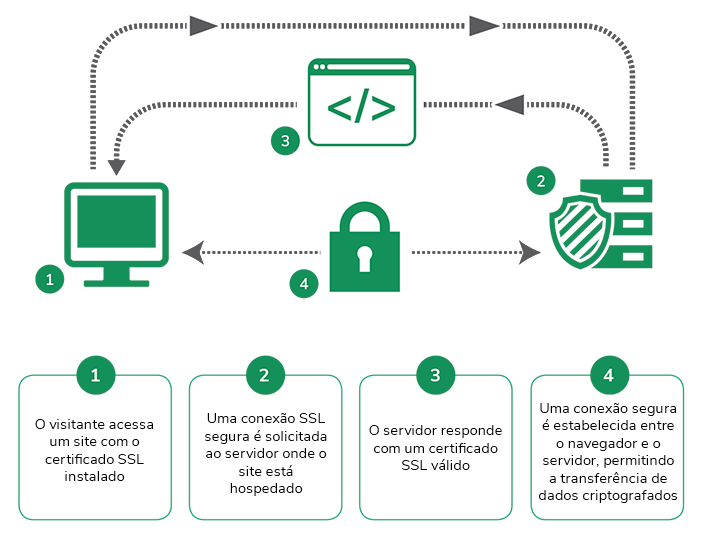
\includegraphics[width=13.5cm]{ssl-funcionamento.png}
\caption{Exemplo de conexão SSL/TLS}
\end{figure}

\subsection{Projeto Let's Encrypt}
\label{cap:lets-encrypt}

A Let's Encrypt é uma autoridade certificadora gratuita, automatizada e aberta que se tornou possível graças a organização sem fins lucrativos \textit{Internet Security Research Group} (ISRG). Seu objetivo, assim como o do protocolo ACME, é tornar possível a configuração de um servidor HTTPS e fazê-lo obter automaticamente um certificado confiável sem intervenção humana. Isso é feito através do uso do agente de gerenciamento de certificado no servidor web.

O certificado é válido por 90 dias, o qual pode ser renovado a qualquer momento. Os certificados são criados através de um processo automatizado, feito  para eliminar a complexidade dos processos atuais de criação, validação, instalação e renovação de certificados para sites seguros. O projeto tem como objetivo fazer com que as conexões criptografadas sejam de fácil acesso para todos os servidores da\textit{World Wide Web}. Ao eliminar barreiras como pagamento e a renovação do certificado, espera-se que a complexidade de manter e configura a criptografia TSL diminua.

\subsection{Protocolo ACME}
\label{cap:prot-acme}

O Ambiente de Gerenciamento de Certificados Automatizados (ACME) é um protocolo padrão para automatizar a validação de domínio, instalação e gerenciamento de certificados X.509. Foi projetado pelo \textit{Internet Security Research Group} (ISRG) para seu projeto \textit{Let's encrypt}. Em resumo, o ACME automatiza as interações entre autoridades certificadoras e os servidores web de seus usuários, permitindo assim o desenvolvimento automatizado de uma infraestrutura de chaves públicas com um custo relativamente baixo.

O ISRG fornece implementações de referência gratuitas e de código aberto para ACME: certbot é uma implementação baseada em Python do software de gerenciamento de certificados de servidor usando o protocolo ACME e boulder é uma implementação de autoridade de certificação escrita em Go. Outras implementações de servidor ACME incluem step-ca de Smallstep e Keyon Enterprise PKI.

\chapter{Primeiro experimento: Preparar um serviço de servidor Web seguro usando certificados Let's Encrypt}
\label{cap:primeiro-experimento}

O experimento foi realizado através da criação de um servidor web com o auxílio dos pacotes \textit{express} e \textit{Node.js}. Também foi criado uma instância de uma máquina virtual (VM) com o sistema operacional (SO) \textit{Debian 10} através do \textit{Compute Engine}, serviço da \textit{Google Cloud Platform} (GCP), o qual é acessível via SSH, possibilitando a execução de comandos em um terminal. Após acessar o terminal do servidor, foi feito a atualização das informações dos pacotes do SO e, na sequência, instalados as ferramentas NVM, npm, \texit{Express}, \textit{Node.js} e \textit{Certbot}.

O \textit{Certbot} é uma ferramente gratuita e \textit{open-source} usada para habilitar HTTPS em websites, de forma automática, usando os certificados \textit{Let's Encrypt}. Essa ferramenta foi usada para geração do certificado SSL. Para isso, foi executado o seguinte comando:
\begin{lstlisting}[language=bash]
  $ sudo certbot certonly --manual
\end{lstlisting}

O terminal então pede para informar um domínio:

\begin{figure}[H]
\centering
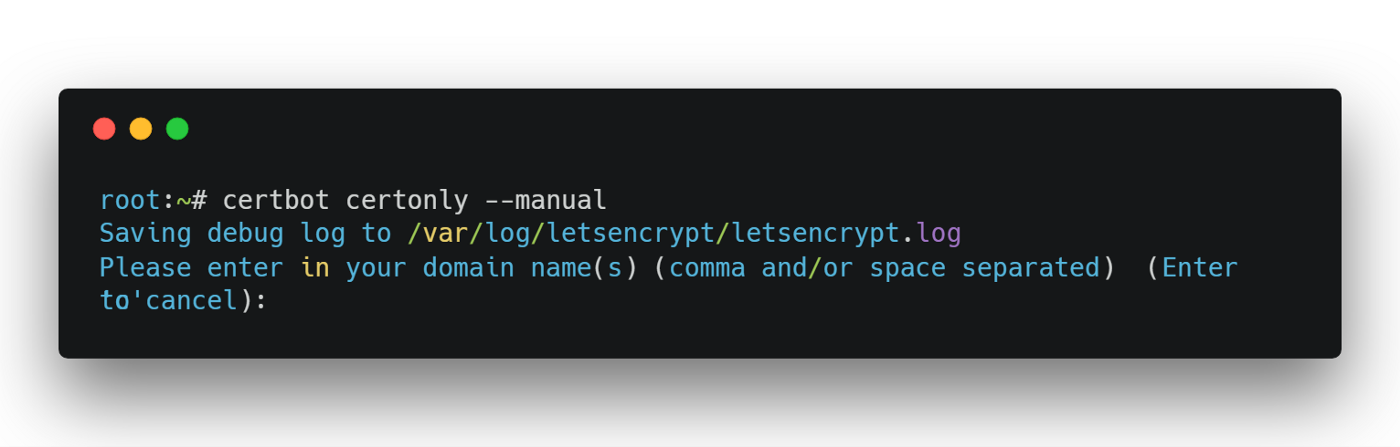
\includegraphics[width=13.5cm]{domain.png}
\end{figure}

E após isso irá pedir a criação de um arquivo chamado \textit{a-string} com o conteúdo \textit{a-challenge}. É necessário criar os diretórios a partir da pasta raiz do servidor. Estes dois nomes acima são só exemplos do que será informado na hora da criação.
\begin{figure}[H]
\centering
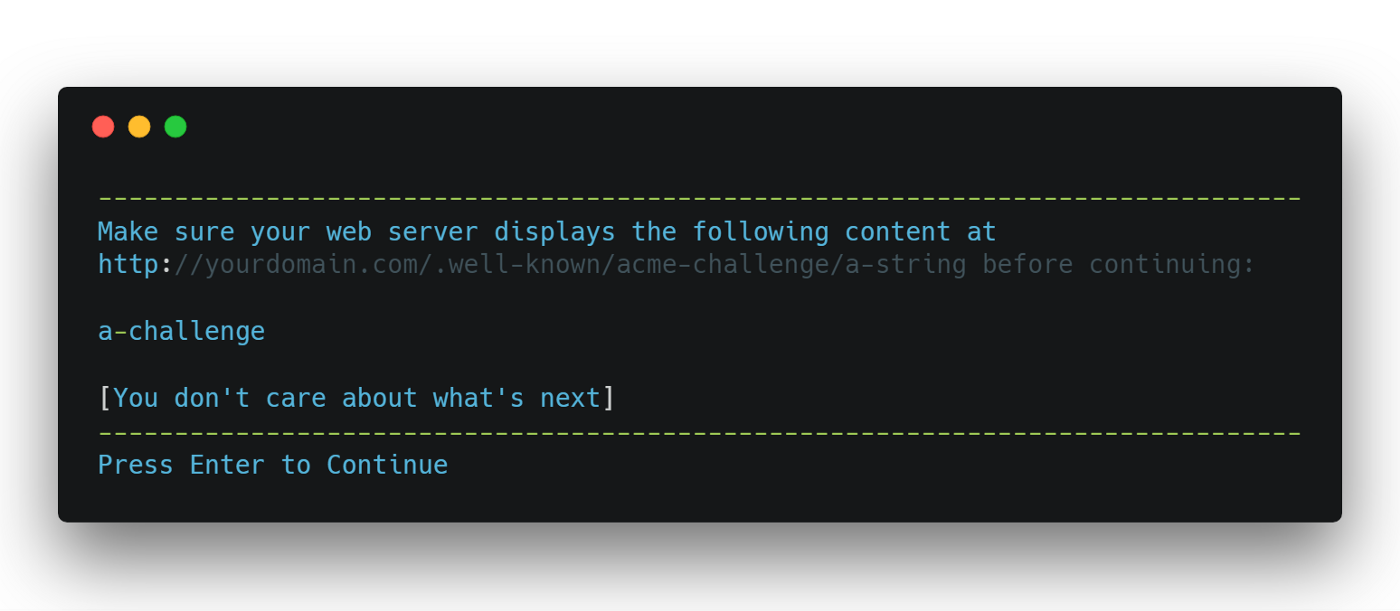
\includegraphics[width=13.5cm]{verify.png}
\end{figure}

Após a criação do arquivo, o IP externo da VM em questão foi associado ao domínio \textbf{trabgrupotlsine.zapto.org}, criado a partir do site \href{https://noip.com}{noip.com}, tornando possível o acesso ao arquivo. Dando continuidade, com a ajuda do \textit{Express} e \textit{Node.js} criou-se um servidor mínimo para tornar possível o acesso a este arquivo. Somente após subir o servidor é que houve a continuação da configuração do certificado SSL via \textit{certbot}. Ao final, é mostrado uma mensagem de sucesso:

\begin{figure}[H]
\centering
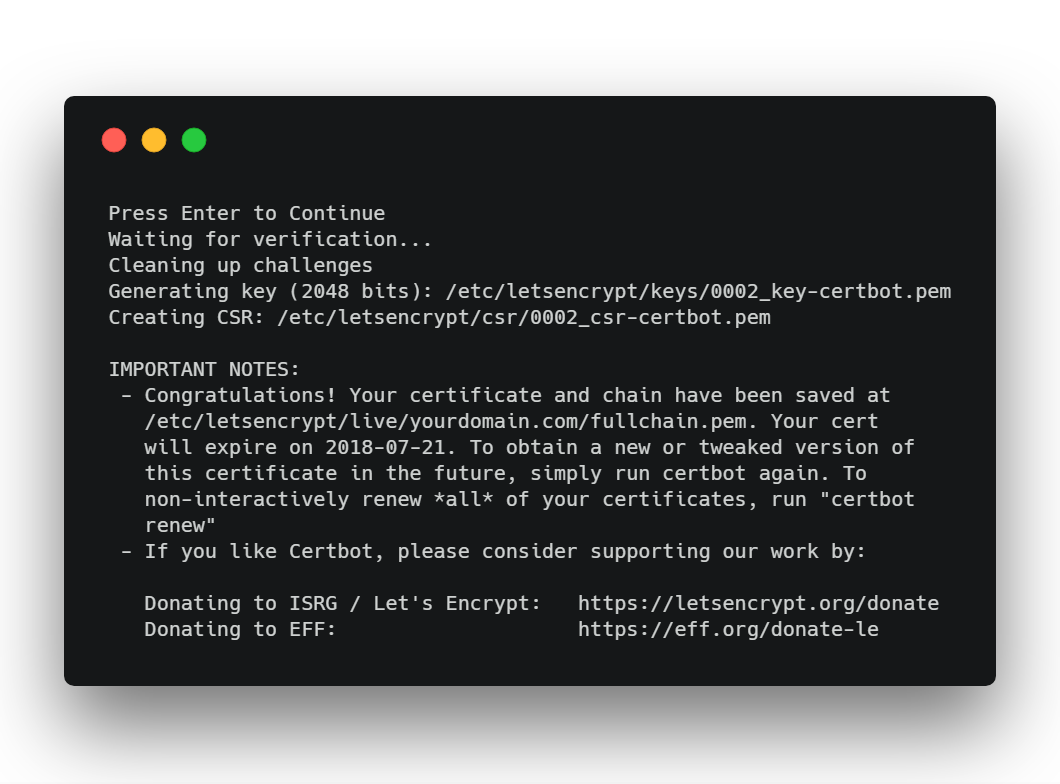
\includegraphics[width=13.5cm]{created.png}
\end{figure}

Ao final, acessando o site \href{https://trabgrupotlsine.zapto.org}{https:// trabgrup otlsine.zapto.org} é possível ver o ícone de cadeado ao lado da \textit{url}, mostrando que a conexão via HTTPS foi feita. O certificado criado para este experimento pode ser conferido através do link \href{https://www.ssllabs.com/ssltest/analyze.html?d=trabgrupotlsine.zapto.org}{https://www.ssllabs.com/ssltest/ana lyze.html?d=trabgrupotlsine.zapto.org}.

\begin{figure}[H]
\centering
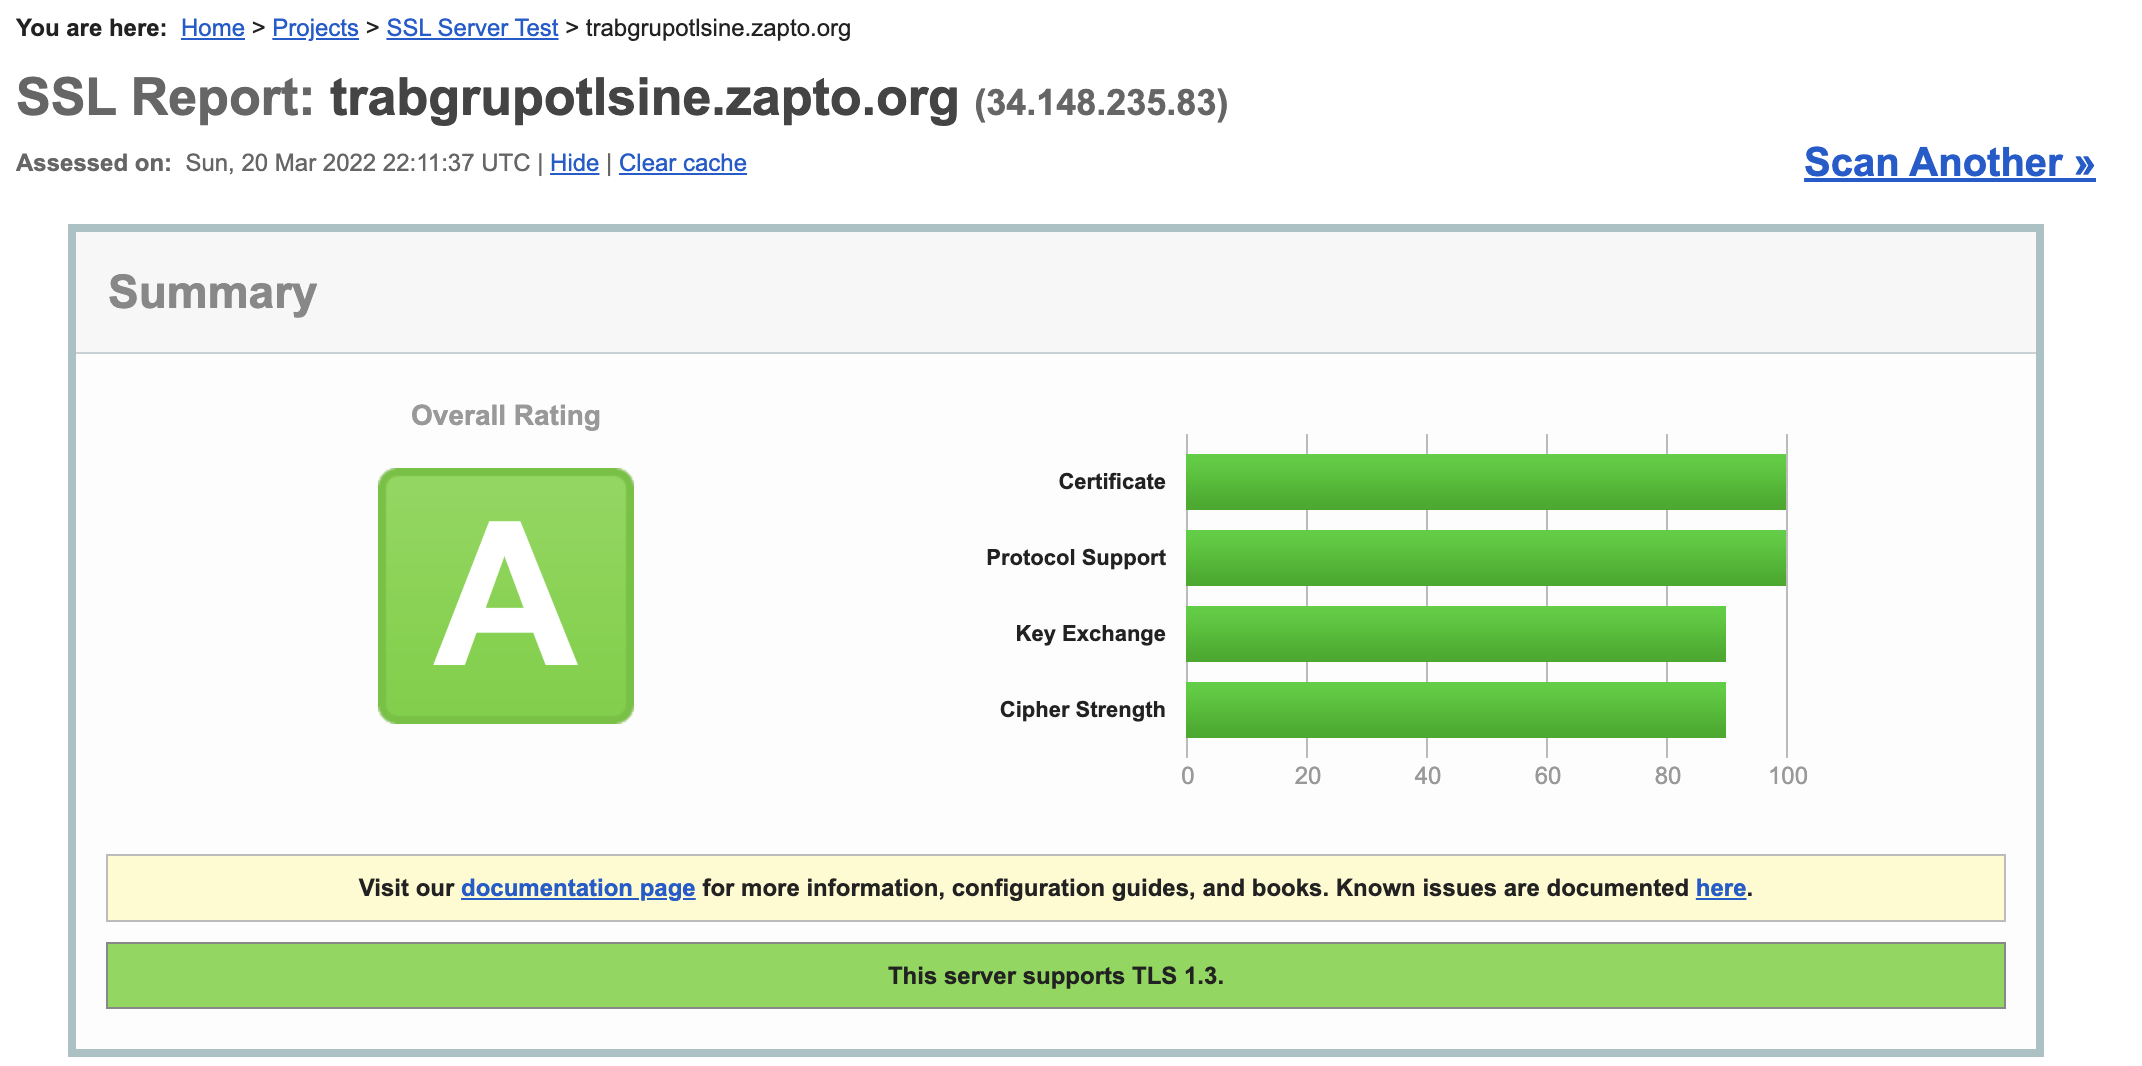
\includegraphics[width=1.1\textwidth]{ssl_verification.png}
\caption{Verificação do SSL no domínio do exemplo}
\end{figure}

\chapter{Segundo experimento: Preparar um serviço proprietário para a renovação automática de certificados TLS proprietários}
\label{cap:primeiro-experimento}

Infelizmente não foi possível realizar o segundo experimento por problemas pessoais e profissionais do autor deste trabalho. 

% ---
% Finaliza a parte no bookmark do PDF, para que se inicie o bookmark na raiz
% ---
\bookmarksetup{startatroot}% 
% ---

% ----------------------------------------------------------
% ELEMENTOS PÓS-TEXTUAIS
% ----------------------------------------------------------
\postextual

% ----------------------------------------------------------
% Referências bibliográficas
% ----------------------------------------------------------
% \bibliography{bibliography}

\end{document}